\chapter{Quantum Computing}
\label{ch:qc}
In this chapter, we provide details of quantum computing and quantum algorithms. Starting by introducing the basic concepts of quantum computing, we then discuss the quantum algorithms used in this thesis. Unlike the previous chapter which provides details of the physics problem we are trying to solve, this chapter focuses on the algorithms and their applications of them. Thus all physical objects such as the Hamiltonian or the Schr{\"o}dinger equation will be treated as pure mathematical objects. 

\section{Qubits}
In analogy to the classical bit, the basic unit of information in classical computing, the basic unit of information in quantum computing is the quantum bit or qubit. A qubit lives in a two-dimensional Hilbert space which can be spanned by two basis vectors, theoretically of choice. Unlike the classical bit, the quantum nature of qubits allows them to be in a superposition of the two basis states. Conventionally, we denote the two basis state as $ \ket{0} $ and $ \ket{1} $, chosen to be the eigenstates of the Pauli-$Z$ operator, such that:
\begin{equation}
	\ket{0} = \begin{pmatrix}
		1 \\
		0
	\end{pmatrix}, \quad
	\ket{1} = \begin{pmatrix}
		0 \\
		1
	\end{pmatrix}.
\end{equation}

The state of a qubit can then be written as a linear combination of the two basis states,
\begin{equation}
	\ket{\psi} = \alpha \ket{0} + \beta \ket{1},
\end{equation}
where $\alpha$ and $\beta$ are complex numbers, with normalisation condition $\alpha^2 + \beta^2 = 1$. 

\subsection{Bloch Sphere}
The state of a qubit can also be represented by a point on the surface Bloch sphere, as shown in Figure~\ref{fig:bloch_sphere}. The Bloch sphere is a unit sphere, where the $ z $ direction the represents the $\ket{0}$ state and the $-z$ direction represents the state $\ket{1}$. Note that although the $x,y$ and $z$ axes are perpendicular in this representation on the Bloch sphere, they are not orthonormal. Vectors pointing at opposite directions are orthonormal, such as the $\ket{0}$ and $\ket{1}$ states.

\begin{figure}[ht]
	\centering
	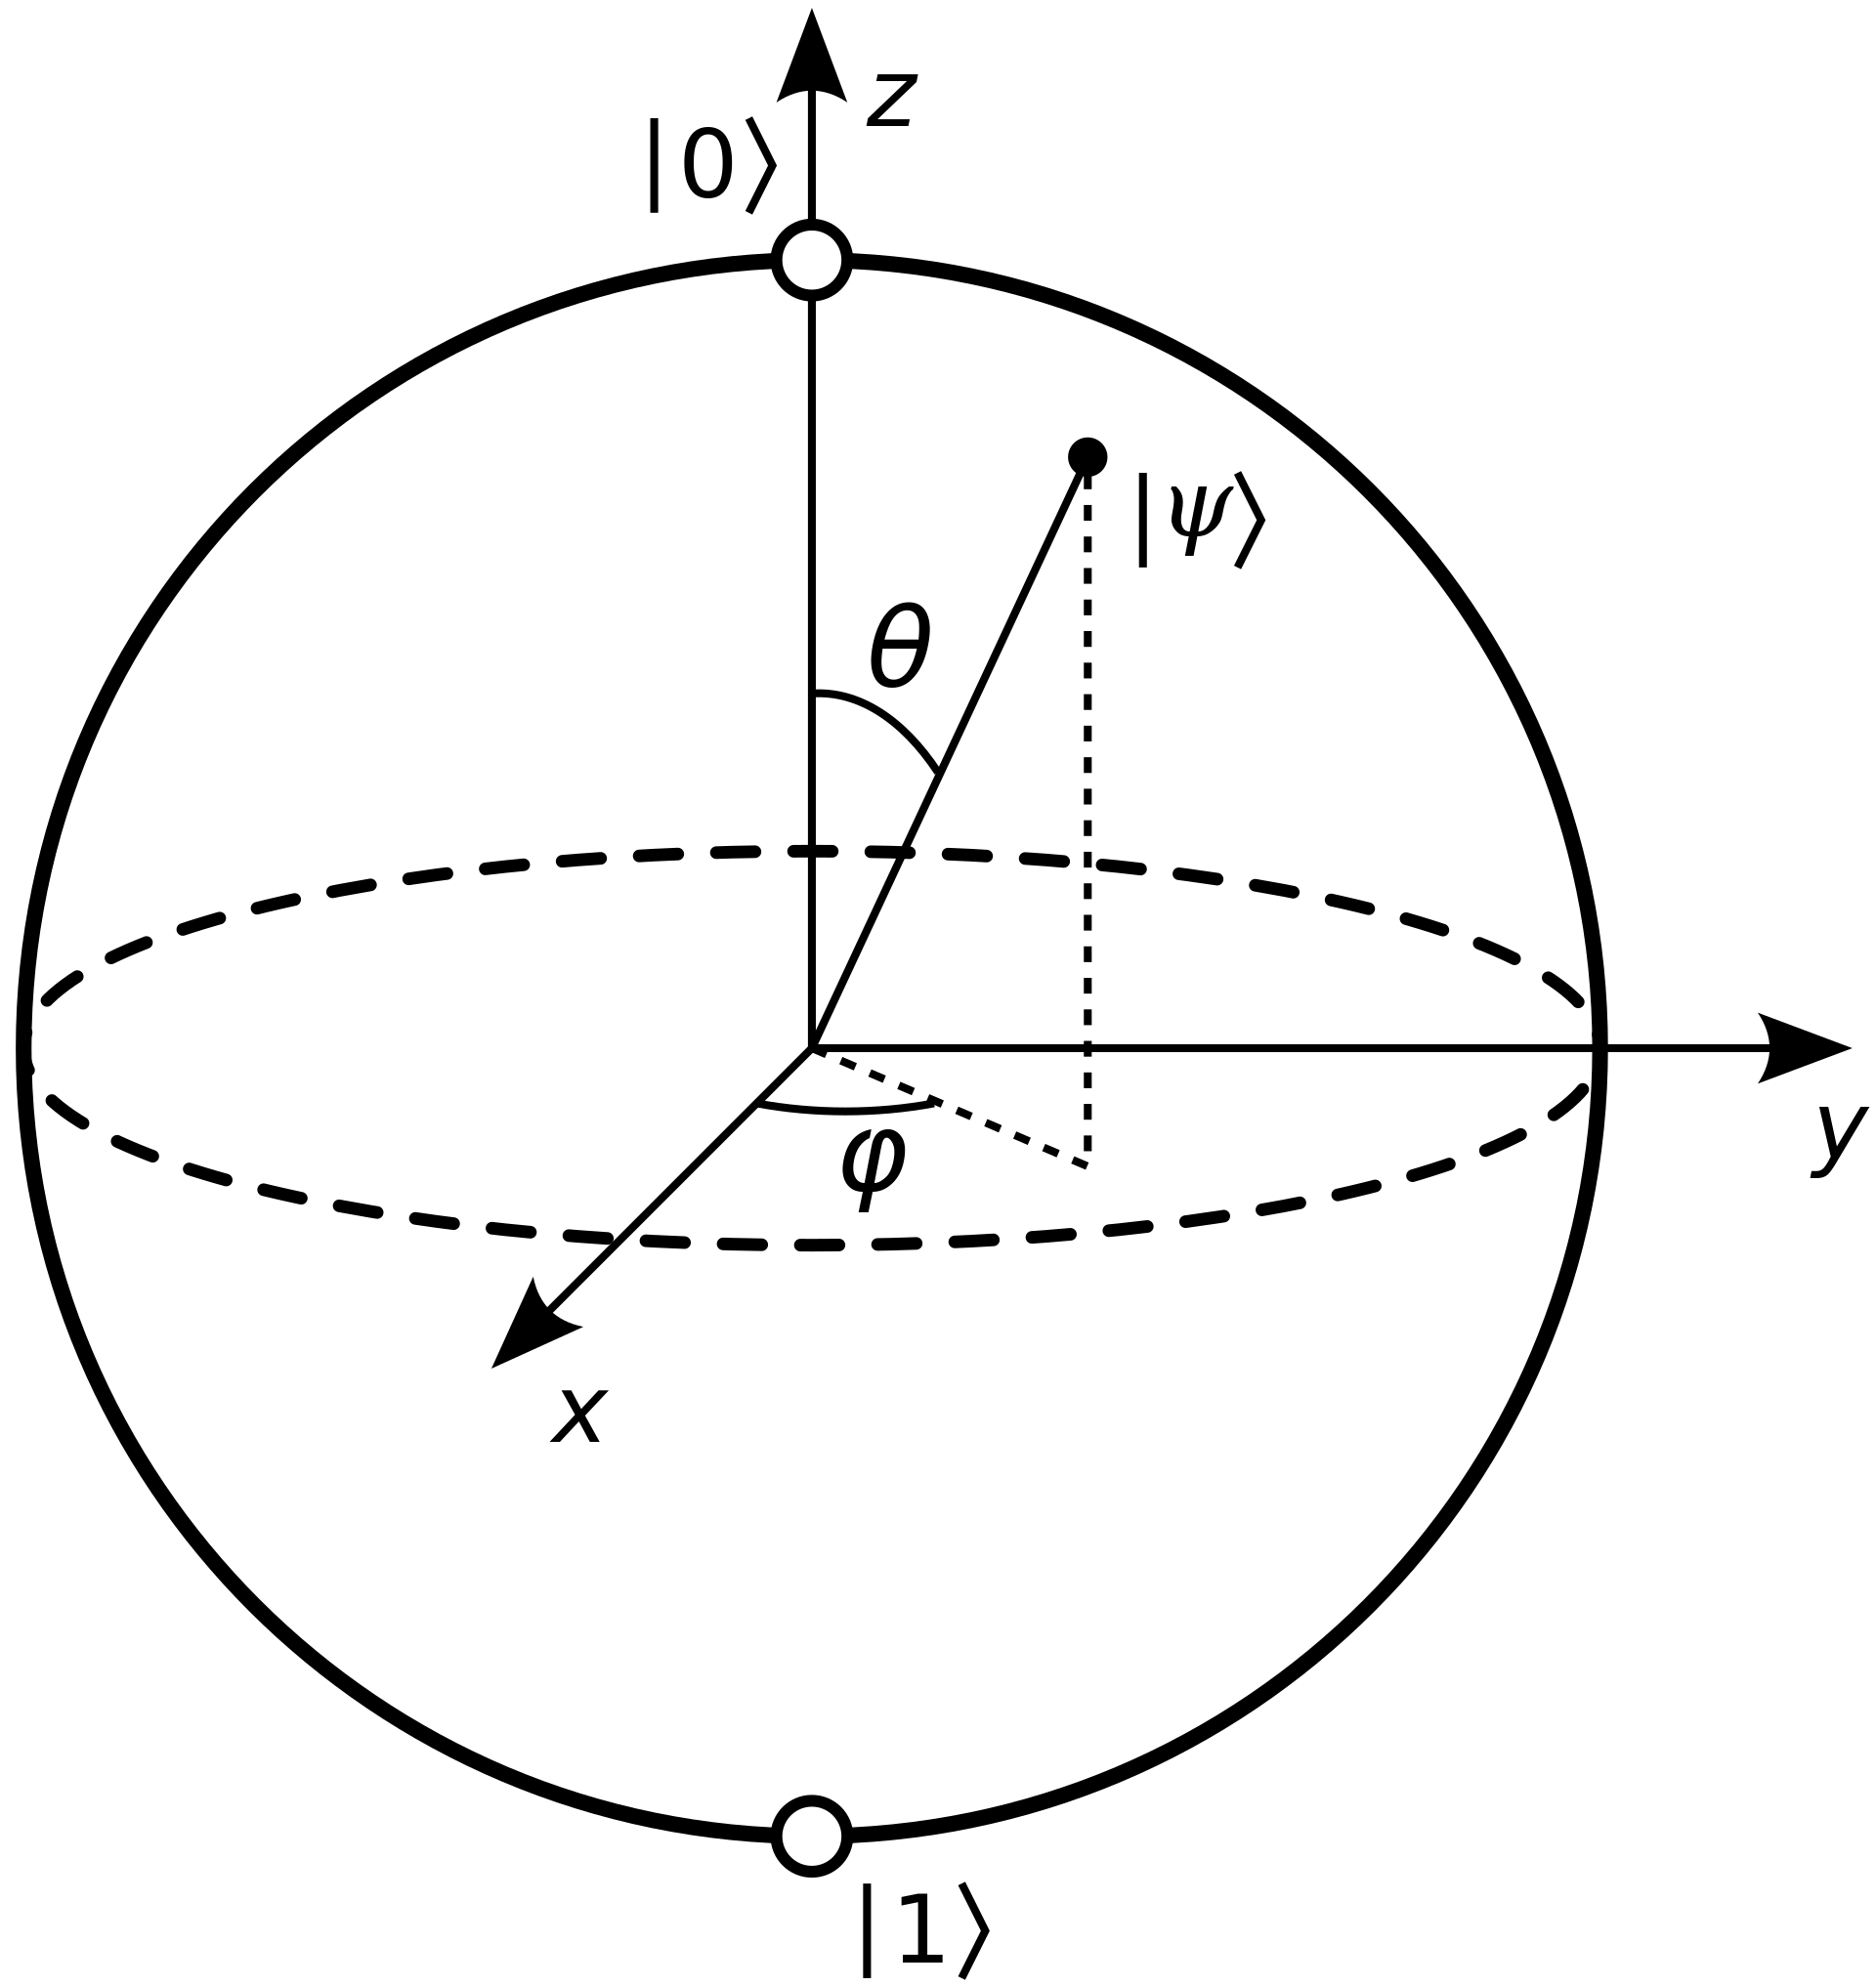
\includegraphics[width=0.5\linewidth]{image/bloch.png}
	\caption{Bloch sphere representation of a qubit. Source: \cite{bloch_sphere_wikipedia}.}
	\label{fig:bloch_sphere}
\end{figure}

\subsection{Multi-qubit State}
Multi-qubit systems are no different from other many-body quantum systems. The combined Hilbert space of $ n $ qubits is the tensor product of the individual Hilbert spaces of each qubit,
\begin{equation}
	\mathcal{H} = \mathcal{H}_1 \otimes \mathcal{H}_2 \otimes \cdots \otimes \mathcal{H}_n.
\end{equation}
The state $ \ket{0 \ldots 0} \equiv \ket{0} \otimes \ket{0} \cdots \ket{0}$ is the tensor product of the $\ket{0}$ states for every Hilbert space. This state is often referred to as the vacuum state of the system. It is worth noting that qubits are assumed to be distinguishable, unlike fermions or bosons. By convention in computer science, the qubit to the right is the first qubit.

\section{Quantum Gates}
\label{sec:quantum_gates}
Mathematically, quantum gates are a series of unitary operators in the operator space $ \mathcal{H} \otimes \mathcal{H}^{*}$ which evolve the state. The unitary nature preserves the norm of the state vector, ensuring the probabilities sum to unity. Since not all gates correspond to an observable, they are not necessarily hermitian. 
\subsection{Single Qubit Gates}
\subsubsection{Pauli Gates}
Pauli gates are Pauli matrices defined in Definition~\ref{def:pauli_matrices}.
\begin{definition}{Pauli Matrices}{pauli_matrices}
    The Pauli matrices are defined as
\begin{equation}
	X \equiv \sigma_x = \begin{pmatrix}
		0 & 1 \\
		1 & 0
	\end{pmatrix}, \quad
	Y \equiv \sigma_y = \begin{pmatrix}
		0 & -i \\
		i & 0
	\end{pmatrix}, \quad
	Z \equiv \sigma_z = \begin{pmatrix}
		1 & 0 \\
		0 & -1
	\end{pmatrix}.
\end{equation}
\end{definition}

The Pauli-X gate is also known as the NOT gate, which flips the state of the qubit.
\begin{align}
	X\ket{0} &= \ket{1}, \\
	X\ket{1} &= \ket{0}.	
\end{align}
The Pauli-Y gate flips the bit and multiplies the phase by $ i $. 
\begin{align}
	Y\ket{0} &= i\ket{1}, \\
	Y\ket{1} &= -i\ket{0}.
\end{align}
The Pauli-Z gate multiplies only the phase of $\ket{1}$ by $ -1 $.
\begin{align}
	Z\ket{0} &= \ket{0}, \\
	Z\ket{1} &= -\ket{1}.
\end{align}

\subsubsection{Hadamard Gate}
The Hadamard gate is defined as
\begin{equation}
	H = \frac{1}{\sqrt{2}} \begin{pmatrix}
		1 & 1 \\
		1 & -1
	\end{pmatrix}.
\end{equation}
It creates a superposition of the $ \ket{0} $ and $ \ket{1} $ states.
\begin{align}
	H\ket{0} &= \frac{1}{\sqrt{2}} \left( \ket{0} + \ket{1} \right), \\
	H\ket{1} &= \frac{1}{\sqrt{2}} \left( \ket{0} - \ket{1} \right).
\end{align}

\subsubsection{Phase Gates}
The S-phase gate is usually denoted as $ S $ and is defined as
\begin{equation}
	S = \begin{pmatrix}
		1 & 0 \\
		0 & i
	\end{pmatrix}.
\end{equation}
It multiplies only the phase of the $ \ket{1} $ state by $ i $.
\begin{align}
	S\ket{0} &= \ket{0}, \\
	S\ket{1} &= i\ket{1}.
\end{align}
Its inverse
\begin{equation}
	S^\dagger = \begin{pmatrix}
		1 & 0 \\
		0 & -i
	\end{pmatrix}
\end{equation}
is known as the $ S^\dagger $ gate which applies a $ -i $ phase shift to \ $ \ket{1}$.
\begin{align}
	S^\dagger\ket{0} &= \ket{0}, \\
	S^\dagger\ket{1} &= -i\ket{1}.
\end{align}

\subsection{Two Qubit Gates}
\subsubsection{CNOT Gate}
\label{ssub:cnot_gate}
The CNOT gate is a two-qubit gate which acts on two qubits, a control qubit and a target qubit. The CNOT gate is defined as
\begin{equation}
	\text{CNOT} = \begin{pmatrix}
		1 & 0 & 0 & 0 \\
		0 & 1 & 0 & 0 \\
		0 & 0 & 0 & 1 \\
		0 & 0 & 1 & 0
	\end{pmatrix}.
\end{equation}
It is often used to perform linear entanglement on qubits.
\begin{align*}
	\label{eq:cnot-behaviour}
	\cnot \ket{00} &= \ket{00}, \\
	\cnot \ket{01} &= \ket{01}, \\
	\cnot \ket{10} &= \ket{11}, \\
	\cnot \ket{11} &= \ket{10}.
\end{align*}
\subsubsection{SWAP gate}%
\label{ssub:swap_gate}
The SWAP gate is a two-qubit gate which swaps the state of two qubits. It is defined as
\begin{equation}
	\text{SWAP} = \begin{pmatrix}
		1 & 0 & 0 & 0 \\
		0 & 0 & 1 & 0 \\
		0 & 1 & 0 & 0 \\
		0 & 0 & 0 & 1
	\end{pmatrix}.
\end{equation}
\begin{align*}
	\swp \ket{00} &= \ket{00}, \\
	\swp \ket{01} &= \ket{10}, \\
	\swp \ket{10} &= \ket{01}, \\
	\swp \ket{11} &= \ket{11}.
\end{align*}


\subsection{Pauli Strings}
A Pauli string, such as $ XIYZ $ is a tensor product of Pauli matrices acting on different qubits. The Pauli string $ XIYZ $ is defined as 
\begin{equation}
	\label{eq:pauli-string-example}
	XIYZ \equiv X_0 \otimes I_1 \otimes Y_2 \otimes Z_3.
\end{equation}
Hamiltonians are often rewritten or decomposed in terms of Pauli string as they can be easily implemented on quantum computers. 

\section{Quantum Circuits}
\label{sec:quantum_circuits}
A quantum circuit is a sequence of quantum gates applied to a set of qubits. 
For example, the Bell state represented by $ \frac{1}{\sqrt{2}} \left( \ket{00} + \ket{11} \right) $  is represented by Figure~\ref{fig:bell_state}~\cite{Nielsen_Chuang_2010}.

\begin{figure}[ht]
	\centering
	\begin{quantikz}
		\lstick{$ \ket{0} $ }  &\gate{H}  &\ctrl{1} &\qw\\
		\lstick{$\ket{0}$}  &\qw   &\targ{} &\qw\\
	\end{quantikz}
	\caption{The quantum circuit which creates the bell state.}
	\label{fig:bell_state}
\end{figure}

\subsection{Quantum Circuit Diagrams}
It is often convenient to represent quantum circuits using quantum circuit diagrams. Table~\ref{tab:qc-diagram} shows the common symbols used to present each component of a quantum circuit.
\begin{table}[ht]
	\centering
	\caption{Quantum Circuit Diagram}
	\label{tab:qc-diagram}

	\begin{tabular}{c c}
		\toprule
	 	Gate & Symbol \\
		\midrule
		$ X $ & \begin{quantikz} & \gate{X} & \end{quantikz} \\
		$ Y $ & \begin{quantikz} & \gate{Y} & \end{quantikz} \\
		$ Z $ & \begin{quantikz} & \gate{Z} & \end{quantikz} \\
		$ H $ & \begin{quantikz} & \gate{H} & \end{quantikz} \\
		$ S $ & \begin{quantikz} & \gate{S} & \end{quantikz} \\
		$ S^\dagger $ & \begin{quantikz} & \gate{S^\dagger} & \end{quantikz} \\
		$ \text{CNOT} $ & \begin{quantikz} & \ctrl{1} & 
					    \\ & \targ{} & \end{quantikz} \\
			$ \text{SWAP} $ & \begin{quantikz} & \swap{1} & \\
					& \targX{} &  \end{quantikz} \\
		\bottomrule
	\end{tabular}
\end{table}


\subsection{Measurement}
\label{sub:measurement}
A measurement is a discontinuous change of the state. A measurement necessarily collapses the state of the qubit to one of the basis states, with probability given by its coefficient. In general, if $  \{ \ket{\psi_j} \} $ is a complete set of basis states, then a measurement on the state $ \ket{\psi} = \sum_{j} c_j \ket{\psi_j} $ in this basis gives a result that can be described as
\begin{equation}
	\ket{\psi} \rightarrow \ket{\psi_j} \quad \text{with probability} \quad |c_j|^2.
\end{equation}
For a product state, the measurement result of any qubit would not affect the states of other qubits, i.e. the probability of each qubit is independent. On an entangled state, for example, a bell state $ \frac{1}{\sqrt{2}} \left( \ket{00} + \ket{11} \right) $, measuring either qubit would collapse the other qubit into the same state. 
The number of times a state is measured in an experiment is commonly known as a ``shot''.

The precision or relative error $ \epsilon $ is defined as 
\begin{definition}{Relative Error}{relative_error}
	If $ a $ is the true value of a quantity and $ a_{meas} $ is the measurement result, then the relative error $ \epsilon $ is defined as 
\begin{equation}
	\label{eq:rel_err}
	\epsilon = \left| \frac{a-a_{meas}}{a} \right|.
\end{equation}
\end{definition}

The number of times a measurement is repeated is called the number of shots. In general, a precision of $ \epsilon $ requires $ \mathcal{O}(1/\epsilon^2) $ shots as a result of statistics~\cite{knill2007}.

\section{Fermionic Encoding}
One key consequence of the Pauli exclusion principle is that no two fermions can occupy the same quantum state, which means a state in a fermionic system can be represented by a binary string. One could map the fermionic creation and annihilation operators to gates as long as the mapping has the same commutation relation.

\subsection{Jordan-Wigner Transformation}
\label{sub:jw}
The Jordan-Wigner transformation is a mapping between fermionic operators and spin operators~\cite{Jordan1993, Seeley2012}. 
If $ \hat a_n^{\dagger} $ is the creation operator for the $n$th fermion,
\begin{equation}
	\label{eq:jw}
	\begin{aligned}	
		\hat a^{\dagger}_n &\mapsto \frac{1}{2} \left[ \prod_{j=0}^{n-1} -Z_j \right] \left( X_n - i Y_n \right), \\
		\hat a_n &\mapsto \frac{1}{2} \left[ \prod_{j=0}^{n-1} -Z_j \right] \left( X_n + i Y_n \right). 
	\end{aligned}
\end{equation}

\subsection{Pauli Decomposition}
The Pauli matrices $\sigma_x (X), \sigma_y (Y), \sigma_z (Z)$, together with the identity operator $ I $ in the space of two by two matrices $ \mathcal{M}_{2\times 2} $ form a complete set of basis in $ \mathcal{M}_{2\times2} $. The tensor products of these operators form complete basiss in the of $ \mathcal{M}_{2^n \times 2^n} $.
If the Hamiltonian $ \hat H $ of a system is given by a $ 2^n \times 2^n $ matrix, 
it could be mapped to qubit space using 
\begin{equation}
	\label{eq:pauli-decomp}
	\hat H_{\text{qubit}} =
	\sum_{\mathcal{P}} \frac{1}{2^n} Tr{\left( \mathcal{P} \hat H \right)},
\end{equation}
where $ \mathcal{P} $ is a Pauli string in $ 2^n \times 2^n $.

This uses only $ \lceil \log_2{n} \rceil $ qubits to map a $ 2^n \times 2^n $ matrix. 


\section{Quantum Algorithms}
\label{sec:quantum_algorithms}

\subsection{Variational Quantum Eigensolver}
\label{sub:vqe}

\begin{figure}[ht]
    \centering
    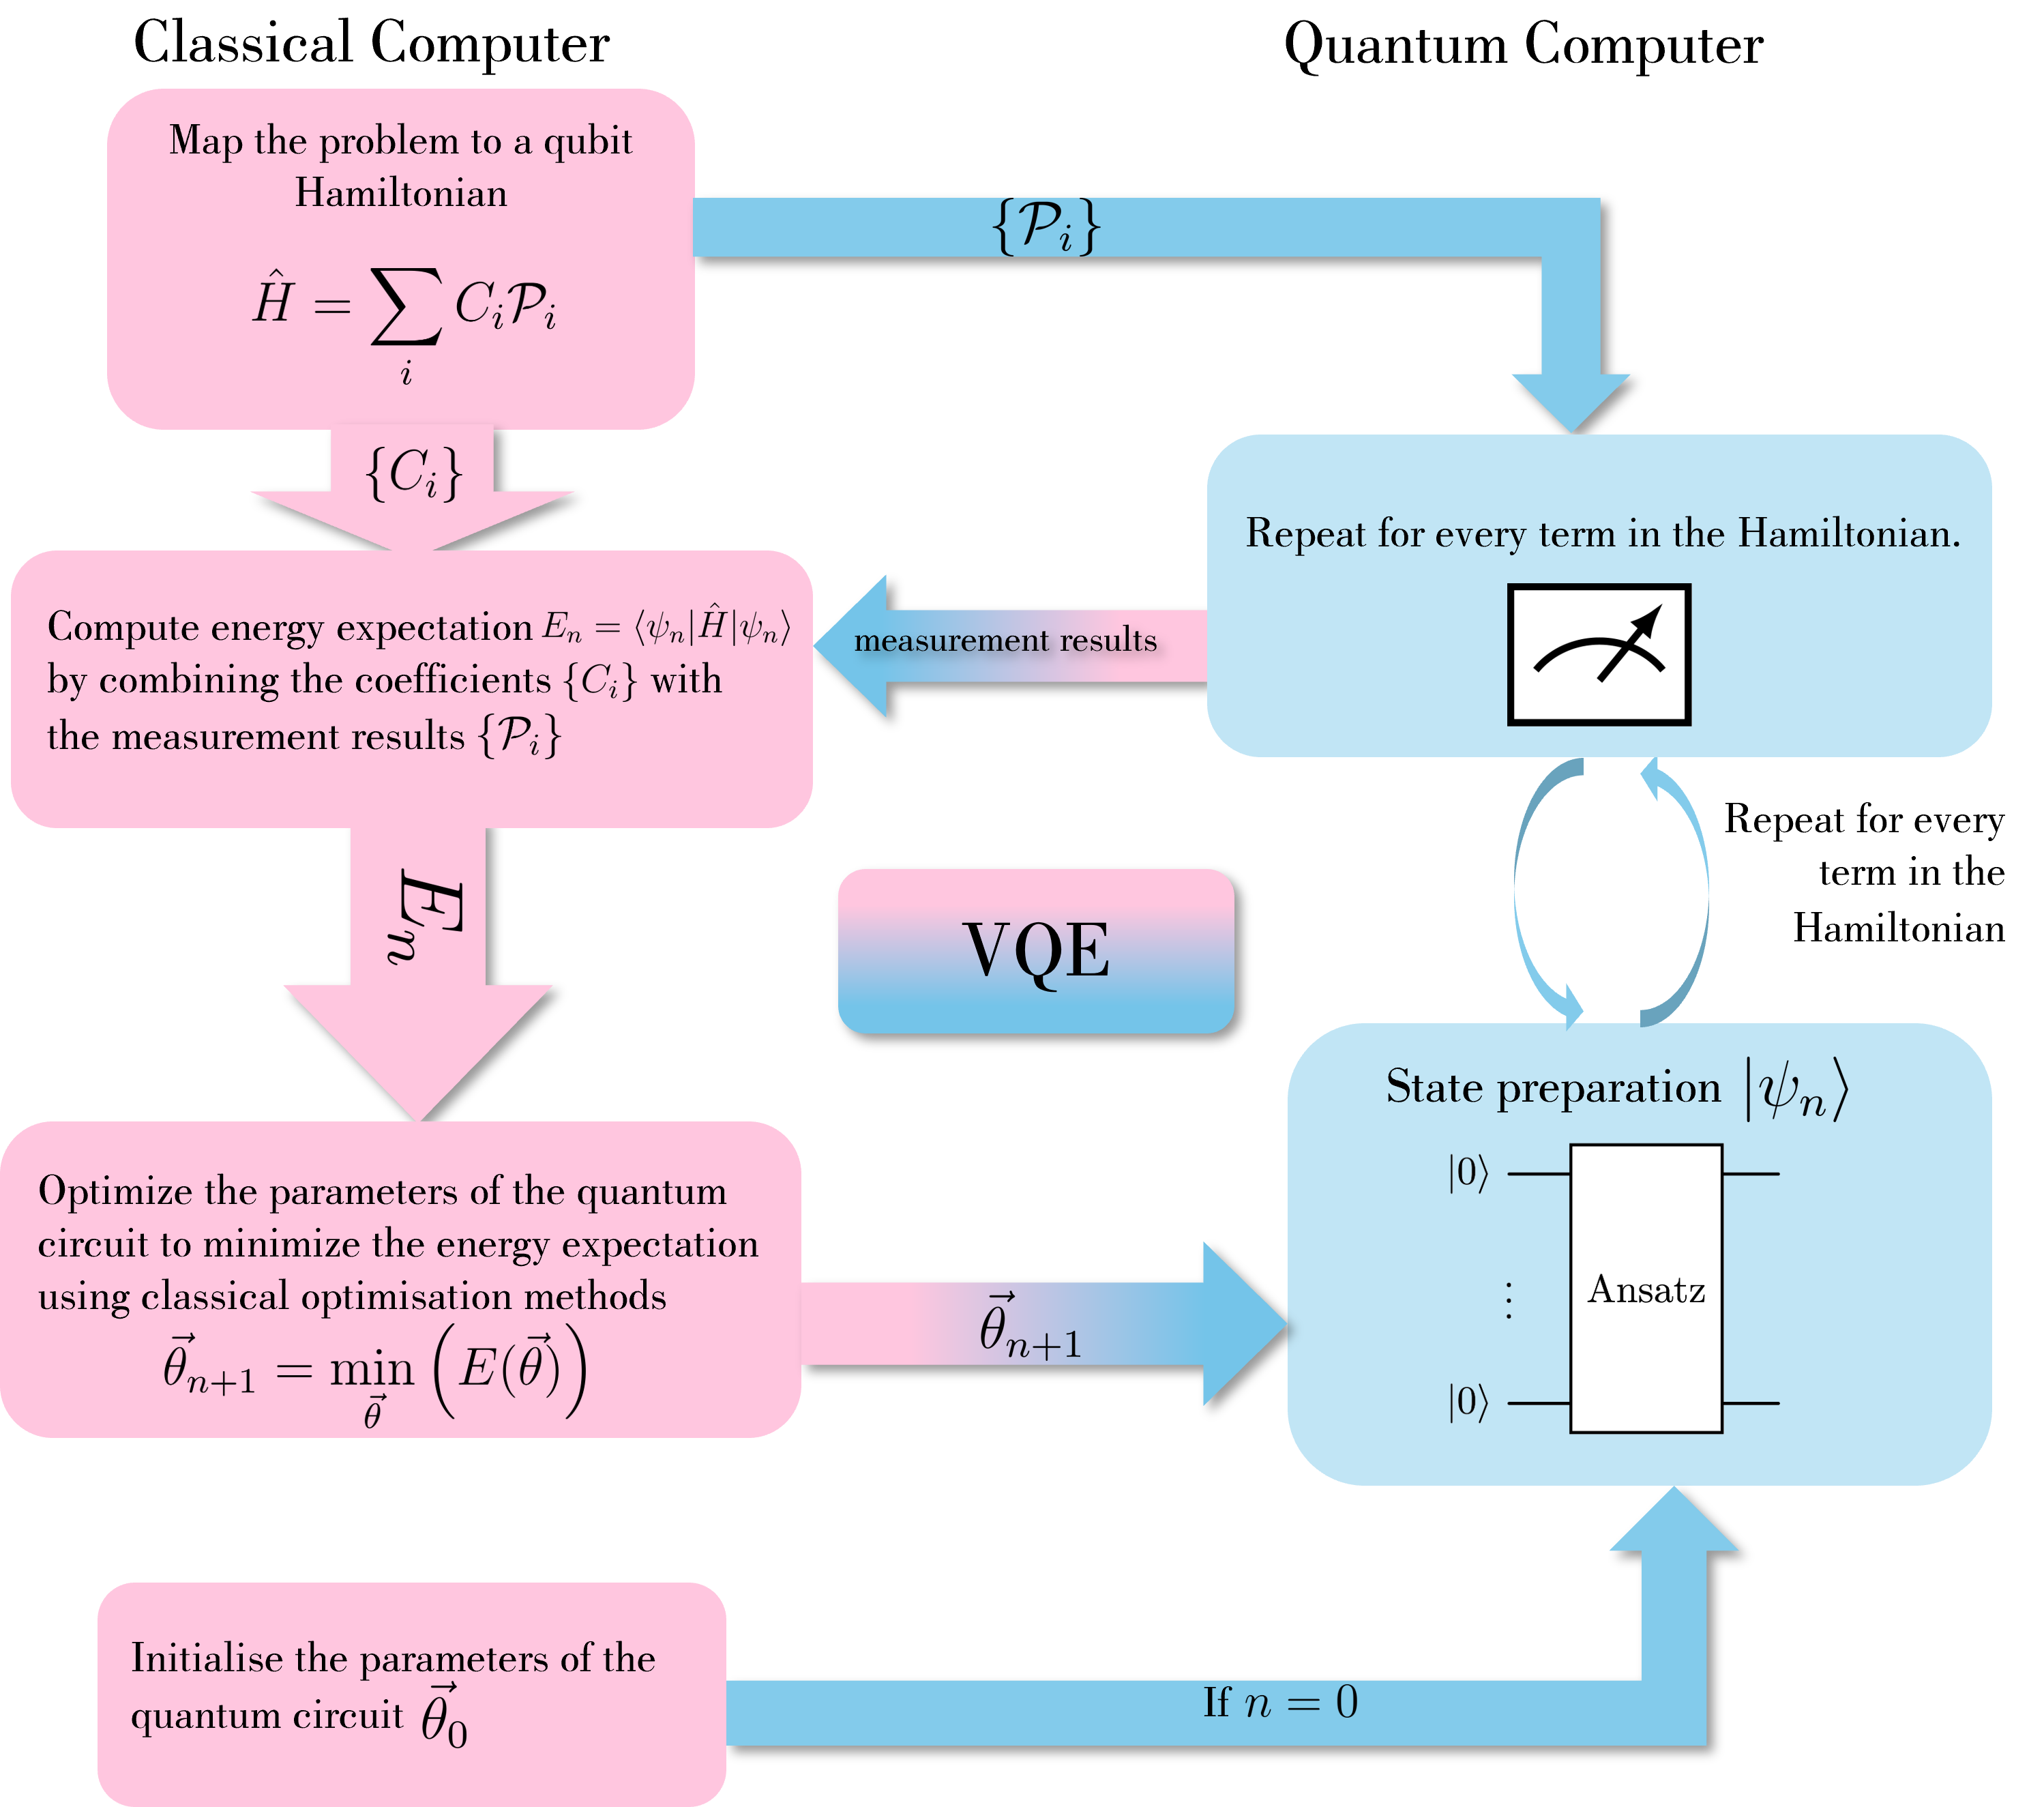
\includegraphics[width=0.7\linewidth]{image/vqe-illu.png}
    \caption{Illustration of the VQE algorithm.}
    \label{fig:vqe-illu}
\end{figure}

The variational quantum eigensolver is a hybrid quantum algorithm that can be realised on a NISQ quantum computer. It consists of an ansatz which is a parameterised circuit. The ansatz prepares a state which is then measured to estimate the energy expectation value. This is the objective function for the classical optimiser which updates the parameter iteratively to find the optimal parameter which minimises the energy utilising the variational principle~\cite{peruzzo2014}. The VQE algorithm is illustrated in Figure~\ref{fig:vqe-illu}. The hybrid and variational nature of the algorithm allows it to be run on NISQ devices and the classical optimisation reduces the length and depth of the quantum circuit.

\subsubsection{Barren Plateaus}
\label{sub:barren_plateaus}
The VQE algorithm amongst many other hybrid quantum algorithms relies on doing optimisation classically and often uses what is called a \textit{Random Parameterised Quantum Circuit(RPQC)} with the form 
\begin{equation}
	\label{eq:rpqc}
	U(\vec{\theta}) = U(\theta_1 \ldots \theta_L) \prod_{l=1}^{L}  U_l(\theta_l) W_l,
\end{equation}
where $ U_l(\theta_l)$ is the parameterised unitary operator of the circuit and $ W_l $ is the unitary operator that does not depend on any parameter. Take the hardware efficient ansatz circuit from Figure~\ref{fig:4hw} as an example: the $ U_l $ would be the single qubit rotation gates and the $ W_l $ would be the CNOT gates, as shown in Figure~\ref{fig:UandW in rpqc}.
\begin{figure}[ht]
	\centering	
	\begin{quantikz}
    \lstick{$q_0$} & \gate{Rx(\theta_0)}\gategroup[4,steps=2,style={inner sep=6pt}]{$U_l$}&\gate{Ry(\phi_0)}&
    \ctrl{1} &\qw &\qw &\qw &\\
\lstick{$q_1$} &\gate{Rx(\theta_1)} &\gate{Ry(\phi_1)} & \targ{}  &\ctrl{1} &\qw &\qw \\
\lstick{$q_2$} & \gate{Rx(\theta_2)} & \gate{Ry(\phi_2)}& \qw &\targ{} &\ctrl{1} &\qw\\
\lstick{$ q_3 $} & \gate{Rx(\theta_3)} & \gate{Ry(\phi_3)}& \qw & \qw & \targ{} &\qw
\end{quantikz}
	\caption{The $ U_l $ and $ W_l $ in a RPQC.}
	\label{fig:UandW in rpqc}
\end{figure}

This is a common form for the ansatz because it allows easy calculations of the gradients
\begin{equation}
	\label{eq:gradient}
	\frac{\partial E\left( \vec{\theta} \right) }{\partial \theta_l} = \frac{\partial \braket{\psi(\vec{\theta})|H|\psi(\vec{\theta})}}{\partial \theta_l} =
	i\braket{0\left|U_{-}^{\dagger}\left[V_k, U_{+}^{\dagger} H U_{+}\right] U_{-}\right| 0},
\end{equation}
where $U_{-} \equiv \prod_{l=0}^{k-1} U_l\left(\theta_l\right) W_l$ and $U_{+} \equiv \prod_{l=k+1}^{L} U_l\left(\theta_l\right) W_l$ \cite{mcclean2018}.
Mcclean et al. also showed that for a large number of random circuits, the average value of the gradient and the variance of the gradient decrease exponentially with the number of qubits~\cite{mcclean2018}. Unlike classical deep neural networks, which scale as $ \mathcal{O}(log(1/\epsilon)) $, the cost of estimating the gradient scales with $ \mathcal{O}(\frac{1}{\epsilon^\alpha})$ where $ \epsilon $ is the deviation from the average value desired and $ \alpha $ is arbitrarily small. The optimisation process is akin to a random walk if $ \epsilon $ is the size of the gradient and the number of measurements is not on the order of $ 1/ \epsilon^{\alpha}$. 
This phenomenon is known as the barren plateau problem, as the gradient has an exponentially small probability of random walking out of the plateau~\cite{mcclean2018}.


\subsubsection{Second Quantised Hamiltonian}%
\label{ssub:second_quantised_hamiltonian}
The Hamiltonians we try to solve with VQE are usually with Hamiltonians in the form of Equation~\eqref{eq:sq_hamiltonian}.

\begin{equation}
	\label{eq:sq_hamiltonian}
	\hat H = \sum_{pq} h_{pq} \hat a_p^\dagger \hat a_q + { \frac{1}{2} \sum_{pqrs} h_{pqrs} \hat a_p^\dagger \hat a_q^\dagger \hat a_r \hat a_s},
\end{equation}
where $ h_{pq} $ and $ h_{pqrs} $ are the one- and two-body integrals, given by 
\[\braket{p|\hat h_0|q}, \] 
and 
\[ \braket{pq|\hat V|rs}, \] 
where $ \hat h_0 $ is the one-body operator and $ \hat V $ is the two-body (interaction) operator.


\subsection{Ansatz}
\label{sub:ansatz}
The form of the ansatz for the VQE is crucial for the convergence of the VQE. A good ansatz should be able to represent the ground state of the system, so that convergence to the ground state energy is possible; span only the necessary section of the Hilbert space, thus reducing the optimisation complexity; as well as be shallow, since we are still in the NISQ era. 

\subsubsection{Hardware Efficient Ansatz}%
\label{ssub:hardware_efficient_ansatz}
A hardware efficient ansatz is a class of ansatzes that uses single qubit rotation gates and linear entanglement CNOT gates that are available to quantum computers~\cite{park2024}. Figure~\ref{fig:4hw} illustrates an example circuit for a hardware efficient ansatz with four qubits. The single qubit rotation gates are parameterised and these parameters are optimised classically to search for the minimum. Note that there could be many other different kinds of hardware efficient ansatz, such as the RyRz ansatz, which uses Ry and Rz gates, or the Ry ansatz, which uses only Ry gates. 
\begin{figure}[ht]
	\centering
	\begin{quantikz}
		\lstick{$q_0$}  &\gate{Rx(\theta_0)}   &\gate{Ry(\phi_0)} &\ctrl{1} &\qw &\qw &\qw &\qw\\
		\lstick{$q_1$}  &\gate{Rx(\theta_1)}   &\gate{Ry(\phi_1)} &\targ{} &\qw &\ctrl{1} &\qw &\qw \\
		\lstick{$q_2$}  &\gate{Rx(\theta_2)}   &\gate{Ry(\phi_2)} &\qw &\qw &\targ{} &\ctrl{1} &\qw\\
		\lstick{$q_3$}  &\gate{Rx(\theta_3)}   &\gate{Ry(\phi_3)} &\qw &\qw &\qw  &\targ{} &\qw \\
	\end{quantikz}
	\caption{Example of the hardware efficient ansatz in a our-qubit circuit.}
	\label{fig:4hw}
\end{figure}

The hardware efficient ansatzes usually have relatively short circuits compared to other ansatzes and are easy to implement on quantum computers since they consist only of gates that are directly available on the hardware. One downside of the hardware efficient ansatz is that there is no information about the Hamiltonian we are trying to solve, and since the ansatz does not exhaust the entire Hilbert space nor should it, it may not be able to represent the ground state of the system. However, it is almost always a good starting point due to the simplicity of the ansatz and serves as a good benchmark for more complex ansatz. 
Although it seems like an ab initio approach, the hardware efficient ansatz can actually successfully represent the ground state of many systems, as we will show in Chapter~\ref{chap:results}. The reason why this worked at all is since the hardware efficient ansatz consists of rotation gates \texttt{Rx, Ry, Rz} and CNOT gates, and these gates form a universal gate set. According to the Solovay-Kitaev theorem, any unitary operator can be approximated to arbitrary precision using a finite number of gates from a universal gate set~\cite{Kitaev1997}. This means that the gates involved in the hardware efficient ansatz can theoretically represent any unitary operator, and thus any state in the Hilbert space. 

\subsection{Adaptive, Problem Tailored VQE}
\label{sub:adapt_vqe}
Grimsley et al. proposed the Adaptive, Problem Tailored VQE (ADAPT-VQE) algorithm~\cite{grimsley2019} which aims to provide an adaptive ansatz structure which can capture information about the Hamiltonian.
The ADAPT-VQE uses an evolving ansatz which is updated at every iteration by appending a new operator onto the circuit chosen from a predefined operator pool without draining the pool. The ADAPT-VQE consists of the following steps:
\begin{enumerate}
	\item Define an operator pool$ \ \{ A \}  $ . 
	\item Calculate the gradient of energy with respect to each operator in the pool.
	\item Select the operator with the largest gradient, $ A $ , append $ e^{\theta A} $ onto the circuit.
	\item Optimise all the parameters in the circuit using VQE.
	\item Repeat steps 2 to 4 until the gradient of all operators is below a threshold.
\end{enumerate}
An ADAPT iteration is defined by steps two to four.
After $ n $ ADAPT iterations, the ansatz should look like:
\[ \ket{\psi_{n}} = e^{\theta_0 A_0} e^{\theta_1 A_1} \ldots e^{\theta_n A_n}\ket{\psi_{0}}. \] 
\subsubsection{Selection Criteria}%
\label{ssub:selectioncriteria}
Steps 2 and 3 of the Adapt VQE require the calculation of the gradient of the energy with respect to the new parameter.
The gradient of the operator $ \left(\frac{\partial E}{\partial \theta}\right)_{\theta = 0} $ is given by:
\begin{align}
	\label{eq:A-gradient}
	\left( \frac{\partial E}{\partial \theta} \right)_{\theta = 0} &= \left( \frac{\partial }{\partial \theta} \right) \braket{\psi_n|e^{-\theta A}H e^{\theta A}|\psi_n}_{\theta = 0}, \\
	&= \braket{\psi_n|\left( -A e^{-\theta A} H e^{\theta A}\right)  + \left( e^{-\theta A}HAe^{\theta A} \right)|\psi_n }_{\theta=0}, \\
	&= \braket{\psi_n|-AH + HA|\psi_n}, \\
	&= \braket{\psi_n|[H,A]|\psi_n}.
\end{align}
The operator $ e^{\theta A_i} $ will be appended if 
\begin{equation}
	\label{eq:selection-criteria}
	\left( \frac{\partial E}{\partial \theta_i}\right)_{\theta_i = 0} > \left( \frac{\partial E}{\partial \theta_j} \right)_{\theta_j = 0}, \quad \forall A_j \in \{A\}. 
\end{equation}
The ADAPT-VQE algorithm is illustrated in Figure~\ref{fig:adapt-illu}.

\begin{figure}[ht]
    \centering
    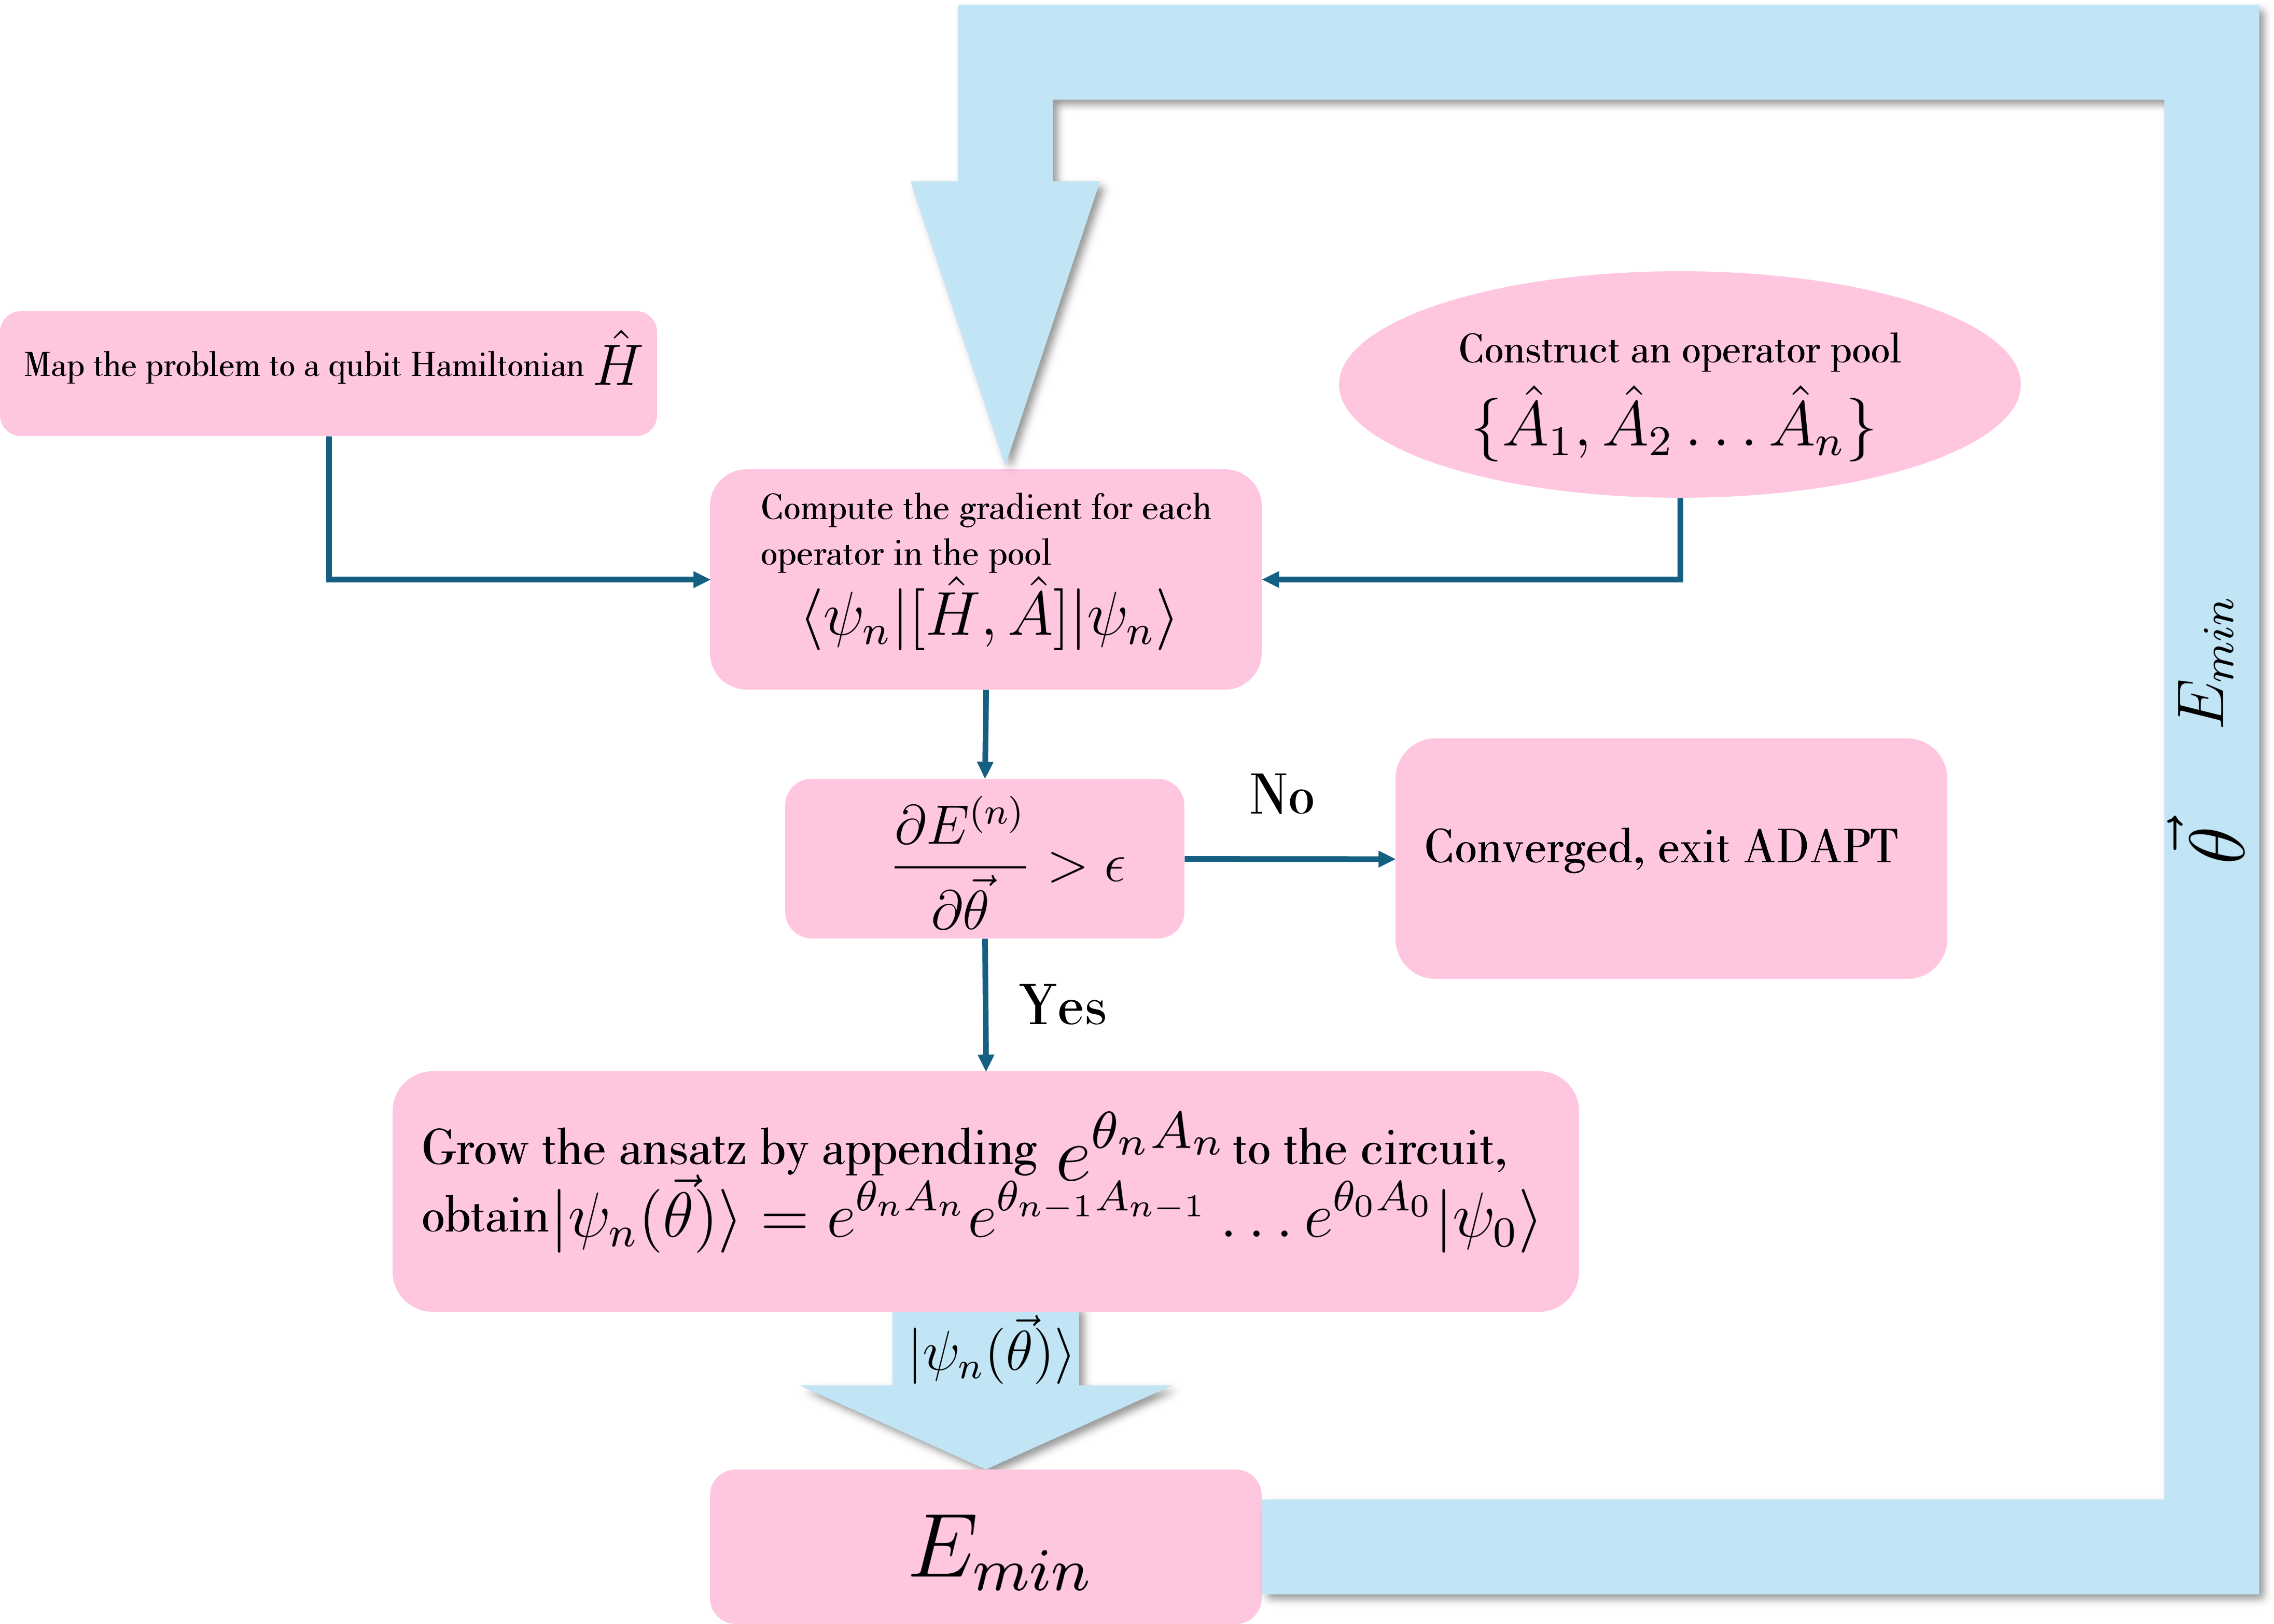
\includegraphics[width=0.8\linewidth]{image/adapt-illu.png}
    \caption{Illustration of the ADAPT-VQE algorithm.}
    \label{fig:adapt-illu}
\end{figure}


\subsection{qubit-ADAPT-VQE}
\label{sub:qubit_adapt_vqe}
The qubit-ADAPT-VQE is a hardware efficient variant of the ADAPT-VQE where the operator pool is chosen to contain only odd Pauli strings, i.e. Pauli strings with odd numbers of Y operators. Since in the case where the Hamiltonian has time-reversal symmetry, the Hamiltonian is real, choosing imaginary Pauli strings causes the analytical expression of the gradient given in Equation~\eqref{eq:A-gradient} to vanish. By choosing only odd operators the ansatz also stays real throughout the ADAPT iterations. A complete pool is defined as a pool that can transform the reference state to any real state. To create any arbitrary real state in the $ n $ qubit Hilbert space requires only $ 2^n -1 $ real parameters.
If $ \{ A_i \}  $ is such that for any arbitrary state $ \ket{\psi}$,  $A_i \ket{\psi}$ form a complete basis, then $ \{ A_i \}  $ is referred to as a complete basis of operators. The minimum size of a complete pool for $ n $ qubit has size $ 2n-1 $, which scales only linearly in number of qubits~\cite{tang2021}. 

We will present the two families of minimal complete pools proven by~\cite{tang2021} and refer to them as the $ V $ pool and $ G $ pool from now on. A family of complete operator pools, $ \{ V_j \}_n $,  where $ V_j $ is an operator in the pool and $ n $ is the number of qubits, can be constructed recursively as follows,
\begin{align}
\label{eq:vpool}
\{ V_j \}_2 = &\{ iY_1Z_2, \ iI_1Y_2 \}, \\
\{ V_j \}_n = &\{\{V_k\}_{n-1}Z_n, \ iI_1I_2 \ldots Y_n, \ iI_1I_2 \ldots Y_{n-1} I_n. \}
\end{align}
	The $ \{ V_j \}_n $ can be mapped onto a different family of operator pool, $ \{ G_j \}_n  $ which contains $ iY $ on every single qubit and two-qubit operator $ iY_kZ_{k+1} $ on adjacent qubits $ k $ and $ k+1 $,  
\begin{align}
\label{eq:gpool}
\{ G_j \}_n = &\{ iY_1I_2 \ldots I_n, \ iI_1Y_2 \ldots I_n, \ \ldots, \ iI_1 \ldots I_{n-1}Y_n, \\
              & iY_1Z_2I_3 \ldots I_n, \ iI_1Y_2Z_3I_4 \ldots I_n, \ \ldots, \ iI_1 \ldots I_{n-2}Y_{n-1}Z_{n}. \}
\end{align}


